\documentclass[11pt]{article}
\usepackage[utf8]{inputenc}
\usepackage[spanish]{babel}
\usepackage{booktabs}
\usepackage{float}
\usepackage[margin=2cm]{geometry}
\usepackage{graphicx}
\usepackage[hidelinks]{hyperref}
\usepackage{longtable}
\usepackage[table]{xcolor}

% --- Paleta (la misma de los informes del Lab 2 y 3) ---
\definecolor{cheapestpink}{HTML}{D6336C}
\definecolor{cheapestdark}{HTML}{A61E4D}
\definecolor{codebg}{HTML}{F4F4F6}
\definecolor{codeborder}{HTML}{9AA0A6}
\definecolor{rowpink}{HTML}{FBEFF3}

\usepackage{titlesec}
\usepackage[labelfont={bf,color=cheapestpink},font=small]{caption}
\usepackage{array}
\usepackage{listings}
\newcolumntype{L}[1]{>{\raggedright\arraybackslash}p{#1}}

\titleformat{\section}
  {\normalfont\Large\bfseries}
  {\colorbox{cheapestpink}{\makebox[1.6em][c]{\color{white}\thesection}}}
  {0.8em}{}
  [{\color{cheapestpink}\titlerule}]
\titleformat{\subsection}
  {\normalfont\large\bfseries\color{cheapestpink}}
  {\thesubsection}{0.8em}{}
\titleformat{\subsubsection}
  {\normalfont\normalsize\bfseries\color{cheapestdark}}
  {\thesubsubsection}{0.6em}{}

\lstdefinestyle{consola}{
  backgroundcolor=\color{codebg},
  rulecolor=\color{codeborder},
  frame=single,
  framerule=0.4pt,
  basicstyle=\ttfamily\small,
  breaklines=true,
  columns=fullflexible,
  keepspaces=true,
  showstringspaces=false,
  xleftmargin=2pt, xrightmargin=2pt,
}
\lstset{style=consola}

\begin{document}

\begin{titlepage}
\centering
\vspace*{3cm}
{\Large\bfseries Experimento de arquitectura:\\[0.3em] Autoescalado de cotización ante campañas de socios\par}
\vspace{1.2em}
{\large Gabriela Hernández -202412025\par}
\vspace{0.3em}
{\color{cheapestdark}\large ISIS-2212 --- Arquitecturas Robustas de Software\par}
\vspace{0.6em}
{\large Solventa --- Fase 1: Monolito Modular\par}
\vspace{1em}
{\color{gray}\itshape Septiembre de 2026\par}
\end{titlepage}

\tableofcontents
\rowcolors{2}{rowpink}{white}
\newpage

\section{El ASR bajo prueba}

\subsection{El escenario}

El escenario que pusimos a prueba es el de una campaña comercial. Un banco aliado lanza una
promoción, y de un momento a otro el tráfico de cotizaciones que nos manda se multiplica por cien:
pasa de 8 cotizaciones por segundo a 830, en menos de un minuto.

\begin{table}[H]
\centering
\begin{tabular}{L{3.2cm} L{12.5cm}}
\toprule
Campo & Contenido \\
\midrule
Fuente & CTO / Arquitectura \\
Estímulo & Que la infraestructura de cotización se autoescale dinámicamente \\
Ambiente & Operación normal \\
Respuesta & Absorber los incrementos drásticos de solicitudes concurrentes provocados por promociones masivas de los bancos aliados \\
Medida & De \textbf{8,3} a \textbf{830} cotizaciones por segundo (factor $\times$100), con una rampa de \textbf{60 s} y \textbf{500 ms} de respuesta bajo carga máxima \\
\bottomrule
\end{tabular}
\caption{El escenario de calidad tal como está registrado en Helix.}
\end{table}

El endpoint que lo materializa es \texttt{POST /cotizaciones}. Ahí pasa el recorrido completo:
se verifica que el cliente tenga consentimiento vigente, se calcula su perfil de riesgo, se aplica
la regla de precio del ramo y se guarda la cotización con su cobertura y su prima.

\subsection{Cómo sabemos si pasa o falla}

Hay un detalle del diseño que define todo el criterio de éxito, y conviene tenerlo claro antes de
leer los resultados: el sistema \textbf{corta por su cuenta} cualquier cotización que tarde más de
medio segundo y responde con un error (HTTP 408). Eso significa que cuando el sistema no da abasto,
no lo vemos como respuestas lentas sino como \textbf{porcentaje de peticiones rechazadas}. Las dos
cosas se midieron, pero el porcentaje de error es el indicador que manda.

\subsection{Lo que esperábamos}

La hipótesis era la más natural: si el tier de aplicación no guarda estado, agregar réplicas
debería dar más capacidad, y entonces bastaría con que la infraestructura las agregue sola cuando
suba la demanda.

\begin{quote}
\textit{Si implementamos elasticidad horizontal automática, entonces \texttt{POST /cotizaciones}
sostendrá 830 cotizaciones por segundo con menos de 500 ms de respuesta dentro del minuto de rampa,
porque el doble de réplicas debería dar el doble de capacidad.}
\end{quote}

Adelanto el final: la hipótesis falló, y falló por dos razones distintas. Pero lo interesante no es
que fallara, sino \textit{por qué}, y eso es lo que el experimento se diseñó para averiguar.

\section{Vistas de arquitectura y tácticas del experimento}

\subsection{Vista de despliegue}

La figura \ref{fig:despliegue} muestra cómo quedó montado el experimento y dónde vive cada táctica
que entró en juego. Es la vista de despliegue del sistema bajo prueba, anotada con los puntos que
medimos.

\begin{figure}[H]
\centering
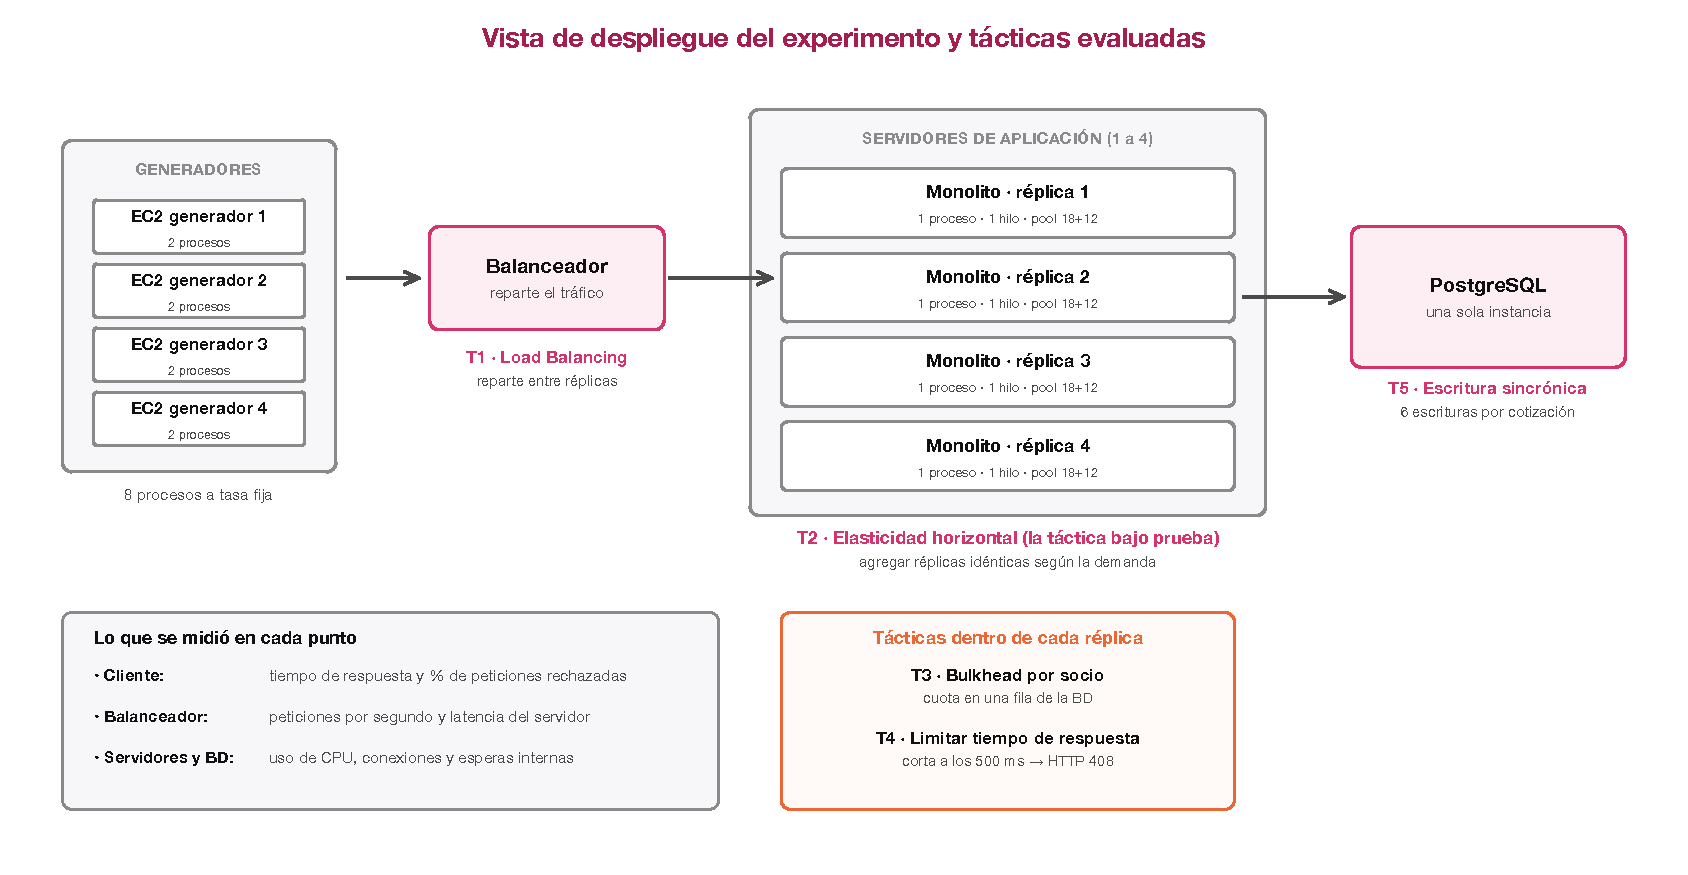
\includegraphics[width=\textwidth]{figuras/fig_despliegue.pdf}
\caption{Vista de despliegue del experimento. Las etiquetas T1 a T5 marcan dónde actúa cada táctica.}
\label{fig:despliegue}
\end{figure}

Vale la pena detenerse en un punto: las cuatro réplicas son idénticas y no guardan nada entre
peticiones, pero \textbf{todas comparten la misma base de datos}. Ese detalle, que en el diagrama
ocupa una sola caja a la derecha, resultó ser el centro de todo el experimento.

\subsection{Las tácticas involucradas}

En el sistema conviven seis tácticas que tocan este escenario. Solo una estaba bajo prueba
(la elasticidad horizontal), pero las otras cinco condicionan el resultado, y algunas de formas que
no habíamos anticipado.

\begin{figure}[H]
\centering
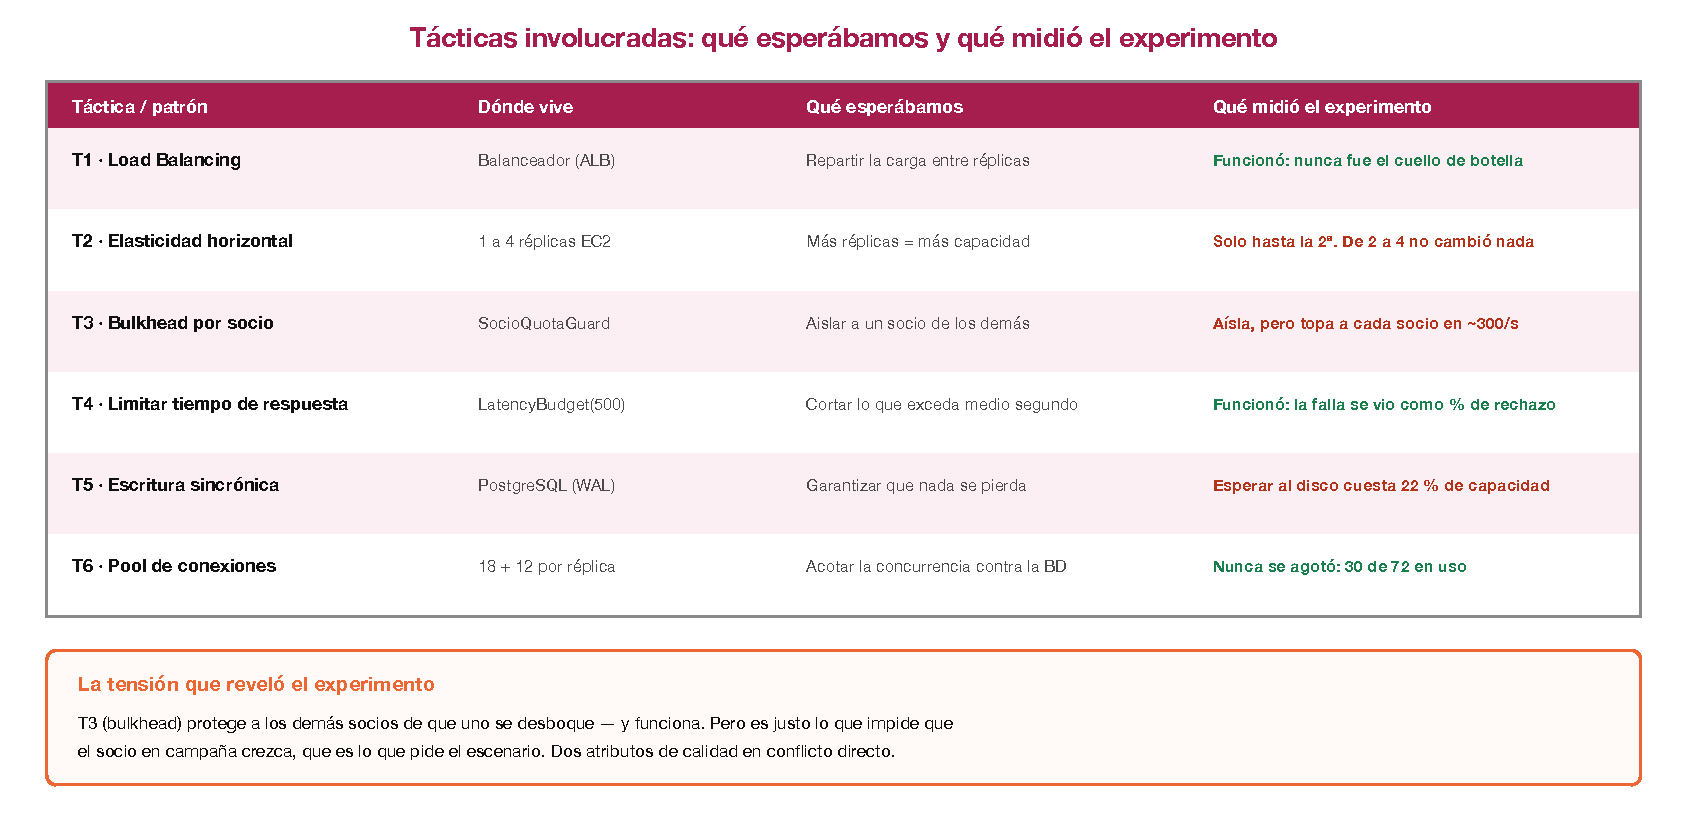
\includegraphics[width=\textwidth]{figuras/fig_tacticas.pdf}
\caption{Las seis tácticas presentes en el escenario, con lo que esperábamos de cada una y lo que
el experimento terminó midiendo.}
\label{fig:tacticas}
\end{figure}

\subsection{Dónde vive cada táctica en el código}

\begin{table}[H]
\centering
\begin{tabular}{L{3.6cm} L{5.2cm} L{7cm}}
\toprule
Táctica & Implementación & Qué hace \\
\midrule
Load Balancing & Application Load Balancer & Reparte las peticiones entre las réplicas sanas \\
Elasticidad horizontal & 1 a 4 instancias EC2 & Agrega o quita réplicas idénticas \\
Bulkhead por socio & \texttt{SocioQuotaGuard} & Cada socio tiene su cuota; si la agota recibe 429 y no afecta a los demás \\
Limitar tiempo de respuesta & \texttt{@LatencyBudget(500)} & Corta la petición que exceda medio segundo \\
Escritura sincrónica & \texttt{synchronous\_commit} de PostgreSQL & Cada confirmación espera a que el dato llegue al disco \\
Pool de conexiones & 18 escritura + 12 lectura por réplica & Acota cuántas consultas simultáneas llegan a la base \\
\bottomrule
\end{tabular}
\caption{Las tácticas presentes en el escenario y su implementación concreta.}
\end{table}

\section{Diseño del experimento}

\subsection{Cómo lo pensamos}

El escenario admite una lectura simple: montar el autoescalado, medir, y listo. El problema es que
esa prueba no responde la pregunta de fondo, que es \textit{si no alcanza, por qué no alcanza}.

Por eso lo armamos como una \textbf{cadena de descarte}: seis etapas, cada una diseñada para
eliminar un sospechoso. Si la capacidad crece con las réplicas, el problema es de velocidad de
reacción; si no crece, el problema está en otro lado y hay que ir a buscarlo. Cada etapa se apoya en
lo que descubrió la anterior.

\subsection{La infraestructura}

\begin{table}[H]
\centering
\begin{tabular}{L{4.5cm} L{2cm} L{9cm}}
\toprule
Para qué & Cuántas & Detalle \\
\midrule
Base de datos & 1 & PostgreSQL 15 en Docker, \texttt{t3.medium}, disco gp3 de 20 GB \\
Aplicación & 1 a 4 & El monolito en Docker, \texttt{t3.medium}, una por zona de disponibilidad \\
Balanceador & 1 & Application Load Balancer, health check en \texttt{/admision/health} \\
Generadores de carga & 4 & \texttt{t3.medium} en la misma región, 2 procesos cada una \\
\bottomrule
\end{tabular}
\caption{Infraestructura del experimento, toda en \texttt{us-east-1}.}
\end{table}


\subsection{La carga de datos}

Una cotización no se puede crear de la nada. Necesita un cliente con consentimiento vigente y un
socio con cuota disponible, porque si falta cualquiera de los dos el sistema la rechaza antes de
llegar al cálculo. Así que antes de medir hay que sembrar datos.

El sembrador (\texttt{seed\_load\_test.py}) los crea \textbf{a través de la API real}, no metiendo
filas a mano en la base. Es más lento, pero garantiza que los datos pasen por las mismas reglas de
negocio que vamos a poner a prueba:

\begin{itemize}
  \item \textbf{200 clientes}, cada uno con su consentimiento vigente.
  \item \textbf{20 pólizas} de muestra.
  \item \textbf{13 socios} con cuota alta (50 millones de solicitudes), para que ninguna corrida se
        detenga porque un socio se quedó sin cupo.
\end{itemize}

Durante la prueba, cada petición se manda a nombre de un cliente y un socio de esas listas, rotando
entre ellos.

\subsubsection{El problema de la acumulación de cotizaciones}

Antes de \textit{cada} corrida hay que borrar las cotizaciones que dejó la anterior. Lo descubrimos
tarde, en las primeras pruebas se acumularon 1,1 millones de cotizaciones, la base se fue poniendo
lenta a medida que crecían sus índices, y el porcentaje de error subió de 35\,\% a 65\,\%
\textbf{sin que cambiáramos absolutamente nada}. Dos corridas idénticas daban resultados distintos
solo por el orden en que se ejecutaron.

Desde entonces el orquestador hace \texttt{TRUNCATE} y \texttt{VACUUM ANALYZE} antes de cada
corrida, y resetea el contador de cuota de los socios.

\subsection{Las etapas y sus parámetros}

\begin{table}[H]
\centering
\small
\begin{tabular}{L{1.1cm} L{4.8cm} L{4.1cm} L{1.5cm} L{1.3cm} L{1.5cm}}
\toprule
Etapa & Qué pregunta responde & Carga & Réplicas & Socios & Repet. \\
\midrule
A & ¿Cuánto aguanta según cuántas réplicas tenga? & 100 a 1000 por segundo, 60 s sostenidos & 1, 2 y 4 & 2 & 3 \\
B & ¿El límite por socio frena el sistema? & 600 por segundo, 60 s & 4 & 1 y 10 & 3 \\
C & ¿Aguanta el pico tal como lo pide el escenario? & 8,3 $\rightarrow$ 832 con rampa de 60 s, 5 min sostenidos & 4 & 2 & 5 \\
D & ¿Mejora si la base no espera al disco? & Igual que C & 4 & 2 & 2 \\
E & ¿Y si no existiera el límite por socio? & Igual que C & 4 & 10 & 2 \\
F & ¿Alcanza con arreglar las dos cosas? & Igual que C & 4 & 10 & 2 \\
\bottomrule
\end{tabular}
\caption{Las seis etapas del experimento. En total 53 corridas y 2 horas 41 minutos de carga efectiva.}
\end{table}

Aparte de las corridas, cronometramos el ciclo completo de encender una réplica nueva: desde que se
pide hasta que el balanceador empieza a mandarle tráfico de verdad.

\subsection{El protocolo de cada corrida}

Para que 53 corridas ejecutadas a lo largo de dos días fueran comparables entre sí, todas pasan por
la misma secuencia, automatizada en \texttt{orquestador.sh}:

\begin{enumerate}
  \item \texttt{TRUNCATE} y \texttt{VACUUM ANALYZE} de las tablas que llena la carga, y reset del contador de cuota.
  \item Verificación del modo de créditos de CPU de la base (las máquinas \textit{burstables} se estrangulan solas si se quedan sin créditos).
  \item Ajuste de cuántas réplicas están registradas en el balanceador.
  \item Inyección simultánea desde los ocho procesos, con la tasa de llegada fija.
  \item Descarga inmediata de los resultados y registro con marcas de tiempo.
\end{enumerate}


\section{Resultados}

\subsection{Etapa A: agregar réplicas no agrega capacidad}

\begin{table}[H]
\centering
\small
\begin{tabular}{r r r r r r r c}
\toprule
Réplicas & Carga pedida & Repet. & Atendió & Típico & 95 de c/100 & Errores & ¿Cumple? \\
\midrule
1 & 100/s & 3 & 96/s & 23 ms & 27 ms & 0,0\,\% & sí \\
1 & 200/s & 3 & 200/s & 25 ms & 30 ms & 0,0\,\% & sí \\
1 & 300/s & 3 & 296/s & 839 ms & 1,4 s & 76,3\,\% & no \\
1 & 400/s & 3 & 400/s & 4,3 s & 7,7 s & 100,0\,\% & no \\
2 & 200/s & 3 & 200/s & 30 ms & 35 ms & 0,0\,\% & sí \\
2 & 400/s & 3 & 400/s & 30 ms & 38 ms & 0,0\,\% & sí \\
2 & 600/s & 3 & 599/s & 969 ms & 8,9 s & 63,1\,\% & no \\
2 & 800/s & 3 & 785/s & 3,3 s & 13,2 s & 69,7\,\% & no \\
4 & 400/s & 3 & 400/s & 29 ms & 54 ms & 0,0\,\% & sí \\
4 & 600/s & 3 & 598/s & 1,1 s & 9,6 s & 55,8\,\% & no \\
4 & 800/s & 3 & 789/s & 2,9 s & 9,3 s & 84,4\,\% & no \\
4 & 1000/s & 3 & 914/s & 3,7 s & 12,2 s & 57,5\,\% & no \\
\bottomrule
\end{tabular}
\caption{Etapa A. Promedio de tres repeticiones por nivel.}
\end{table}

\begin{figure}[H]
\centering
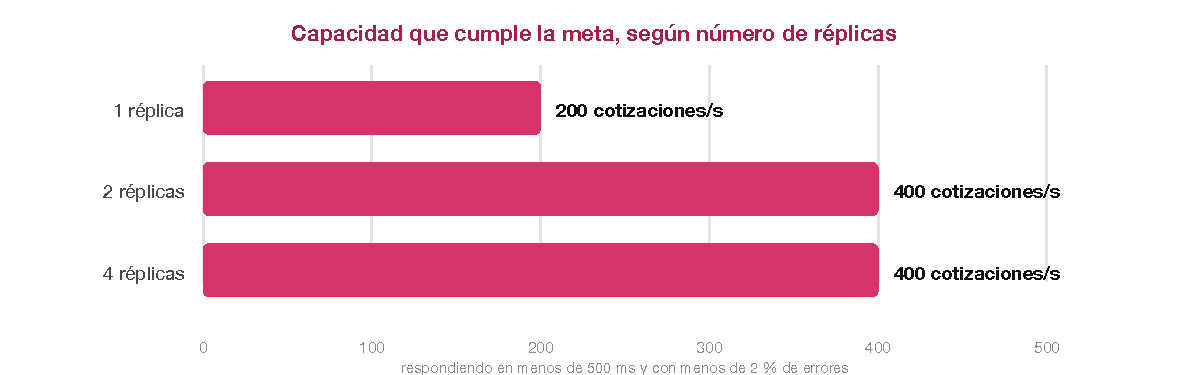
\includegraphics[width=0.85\textwidth]{figuras/fig_capacidad.pdf}
\caption{La capacidad se duplica de una a dos réplicas, y después se queda quieta.}
\label{fig:capacidad}
\end{figure}

Este es el resultado central del experimento. De una réplica a dos, la capacidad se duplicó
limpiamente. De dos a cuatro, \textbf{no se movió}: las dos configuraciones cumplen a 400 por
segundo y las dos se rompen a 600.

Durante esas corridas, las réplicas de aplicación
estuvieron entre \textbf{27\,\% y 38\,\% de uso de CPU}. No les faltaba potencia. Estaban esperando.

\subsection{Etapa B: un solo socio no puede crecer}

\begin{table}[H]
\centering
\begin{tabular}{l r r r r}
\toprule
Reparto del tráfico & Atendió & Tiempo típico & 95 de c/100 & Errores \\
\midrule
Todo de \textbf{1 socio} & 595/s & 4.250 ms & 11,3 s & 89,9\,\% \\
Repartido entre \textbf{10 socios} & 600/s & \textbf{38 ms} & 2,7 s & \textbf{0,5\,\%} \\
\bottomrule
\end{tabular}
\caption{Etapa B. Misma carga de 600 por segundo, misma infraestructura, tres repeticiones cada una.}
\end{table}

\begin{figure}[H]
\centering
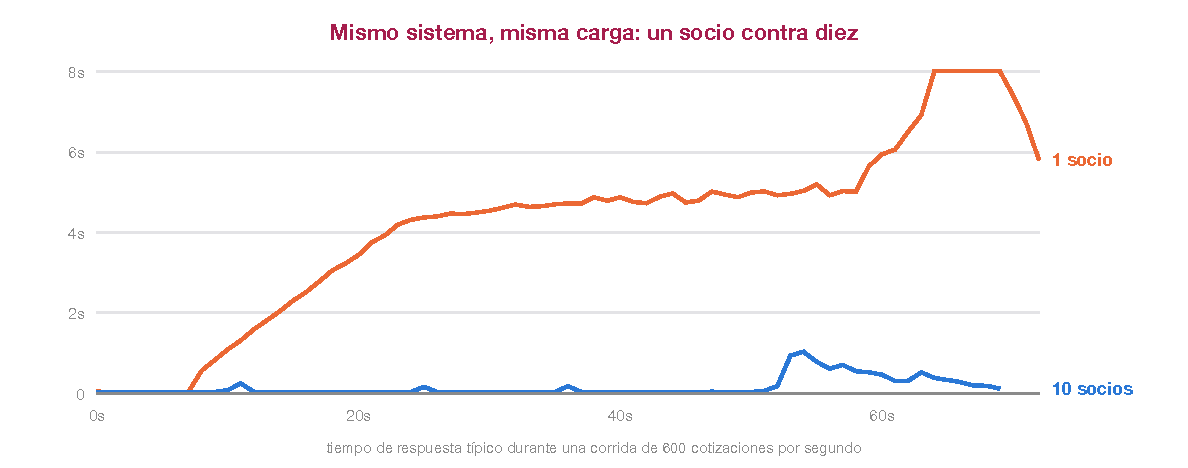
\includegraphics[width=0.85\textwidth]{figuras/fig_socios.pdf}
\caption{Cómo evoluciona el tiempo de respuesta durante la corrida. Lo único que cambia entre las
dos líneas es entre cuántos socios se reparte el mismo tráfico.}
\label{fig:socios}
\end{figure}

Dos órdenes de magnitud de diferencia, con el mismo hardware y la misma carga. La causa es el
contador de cuota: cada cotización actualiza el renglón de su socio en la base, y PostgreSQL obliga
a que las actualizaciones al mismo renglón se hagan de a una. Es una puerta giratoria por la que
solo cabe una persona a la vez, y da igual cuántas entradas tenga el edificio.

Esto es lo más grave para nuestro escenario, porque el escenario dice que \textbf{un socio} lanza la
promoción. Las 830 cotizaciones por segundo vienen todas por esa misma puerta.

\subsection{Etapas C a F: el pico y los intentos de arreglarlo}

\begin{table}[H]
\centering
\begin{tabular}{l r r r r}
\toprule
Escenario & Repet. & Atendió & Tiempo típico & Errores \\
\midrule
C --- como está hoy & 5 & 488/s & 4,3 s & 33,1\,\% \\
D --- sin esperar al disco & 2 & 587/s & 2,8 s & 6,3\,\% \\
E --- repartido en 10 socios & 2 & 603/s & 2,6 s & 11,8\,\% \\
F --- las dos cosas juntas & 2 & 608/s & 2,9 s & 7,2\,\% \\
\bottomrule
\end{tabular}
\caption{El pico del escenario (832 por segundo con rampa de 60 s) bajo cuatro configuraciones.}
\end{table}

\begin{figure}[H]
\centering
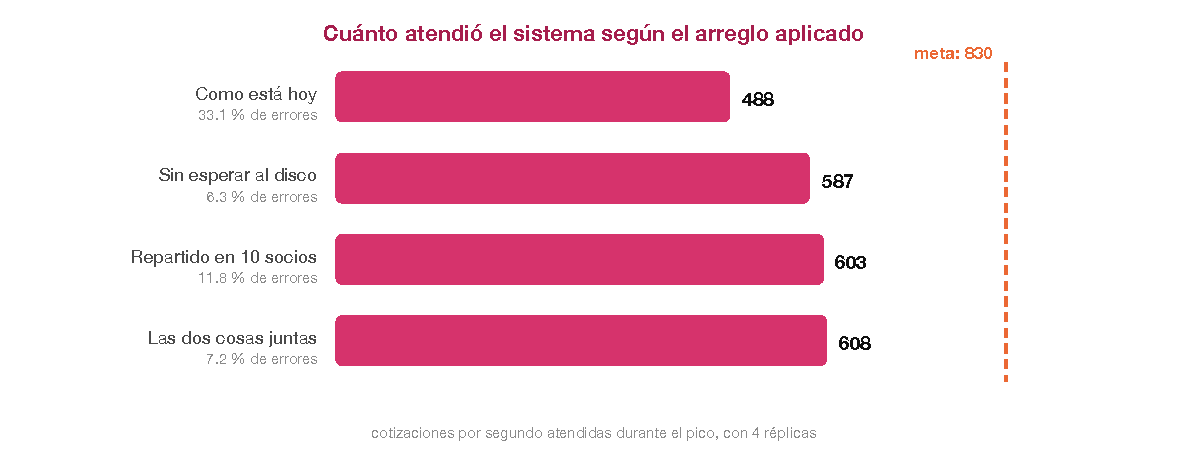
\includegraphics[width=0.85\textwidth]{figuras/fig_mitigaciones.pdf}
\caption{Ninguna combinación se acerca a la meta. Los arreglos bajan mucho los errores, pero el
techo apenas se mueve.}
\label{fig:mitigaciones}
\end{figure}

\subsection{Cuánto tarda en aparecer una réplica nueva}

Cronometramos el ciclo completo: \textbf{81 segundos} desde que se pide la máquina hasta que el
balanceador le manda tráfico. Se reparten así: 18 segundos en encender, y 63 más en instalar
Docker, descargar los 424 MB de la imagen, arrancar la aplicación y pasar dos chequeos de salud
seguidos.

El escenario concede 60 segundos para absorber todo el pico. Y esos 81 segundos son solo el
arranque: falta sumarle el tiempo que tarda Amazon en darse cuenta de que el tráfico subió, que
son otros uno a dos minutos porque las métricas del balanceador se publican en ventanas de un
minuto.

\subsection{Evidencia de la infraestructura}

\begin{figure}[H]
\centering
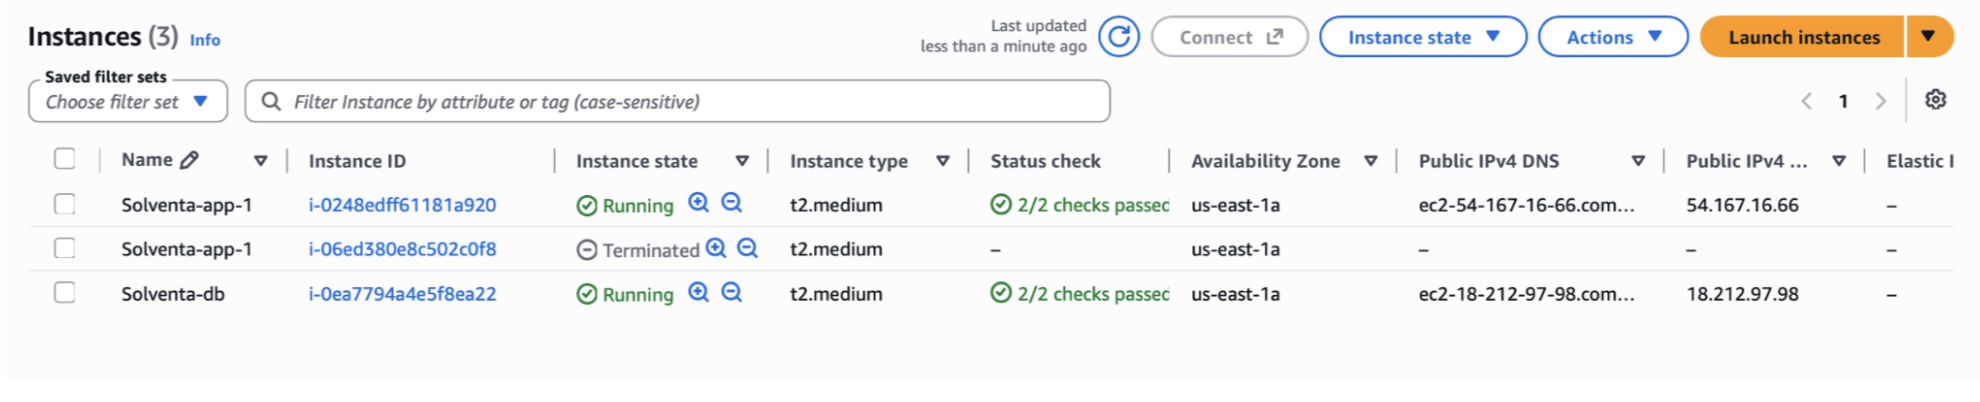
\includegraphics[width=0.92\textwidth]{figuras/Instancias.png}
\caption{Las instancias del experimento en la consola de AWS.}
\end{figure}

\begin{figure}[H]
\centering
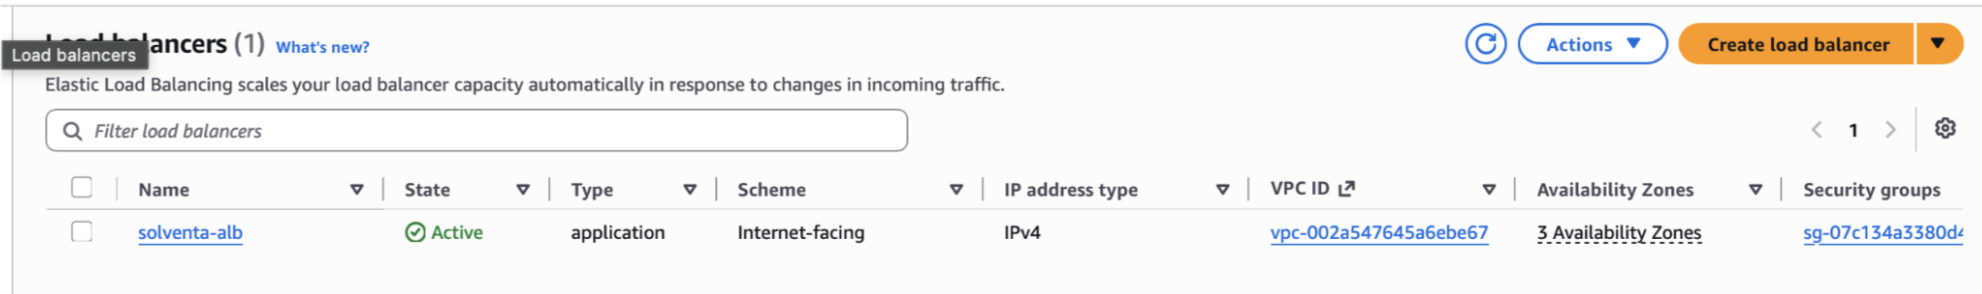
\includegraphics[width=0.92\textwidth]{figuras/BalanceadorCarga.png}
\caption{El balanceador de carga que reparte el tráfico entre las réplicas.}
\end{figure}

\begin{figure}[H]
\centering
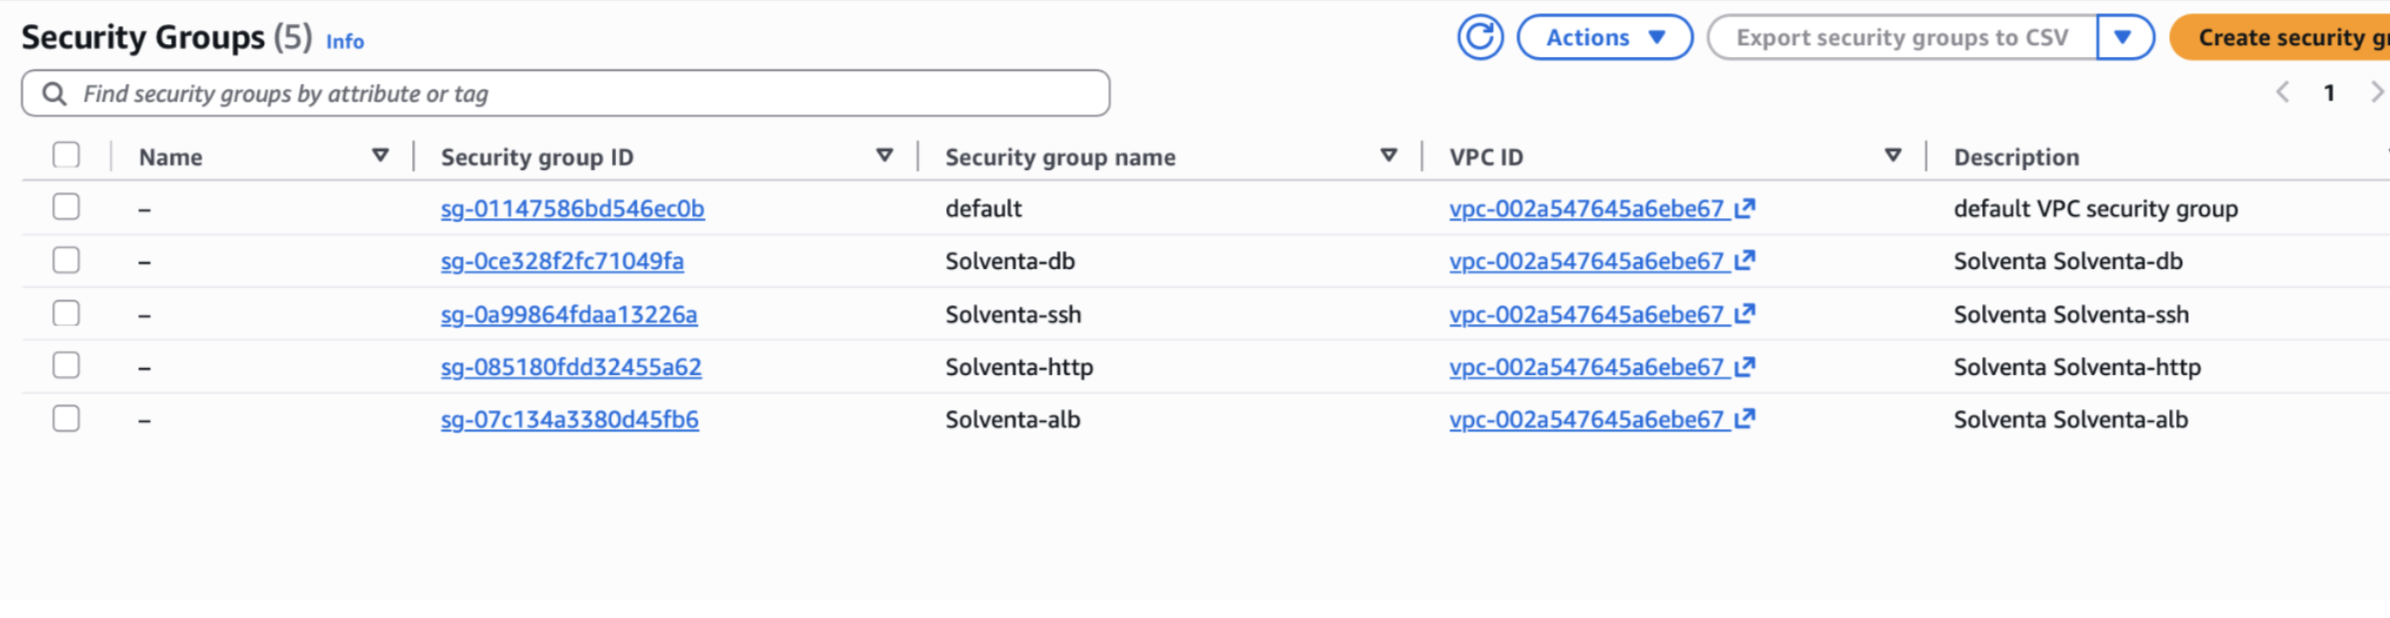
\includegraphics[width=0.92\textwidth]{figuras/SecurityGroups.png}
\caption{Los grupos de seguridad que habilitan el tráfico entre las capas.}
\end{figure}

\section{Análisis de resultados}

\subsection{El cuello de botella es la base de datos}

Todos los números apuntan al mismo lugar. Mientras el sistema se ahogaba atendiendo 488 cotizaciones
por segundo y rechazando un tercio de ellas, las réplicas de aplicación estaban al 30\,\% de uso y
solo 30 de las 72 conexiones disponibles estaban ocupadas. No les faltaba capacidad: esperaban a la
base.

Se confirma al comparar configuraciones. Pasar de una a dos réplicas duplicó la capacidad, porque
ahí la aplicación sí era el límite. Pasar de dos a cuatro no cambió nada, porque a partir de ese
punto el recurso limitante pasó a ser la única instancia de PostgreSQL que todas comparten.

Sirve la imagen del restaurante: contratar un segundo mesero duplica la atención mientras los
meseros sean el cuello. Pero cuando la cocina es la que no da más, se pueden contratar diez y los
platos no salen más rápido.

\subsection{Por qué espera la base}

Fuimos a mirar directamente qué estaba haciendo PostgreSQL durante la saturación, y encontramos dos
esperas:

\begin{itemize}
  \item \textbf{La escritura al disco.} Cada confirmación de transacción espera a que el dato quede
        escrito en el registro de la base, y eso cuesta 0,94 milisegundos por operación. Parece poco,
        pero a cientos de transacciones por segundo se convierte en una fila.
  \item \textbf{El renglón del contador de cuota.} Todas las cotizaciones de un mismo socio compiten
        por actualizarlo, y se procesan de a una.
\end{itemize}

No era la CPU de la base (que llegó al 72\,\%, alto pero no saturado), no era el disco por falta de
capacidad (209 operaciones por segundo de las 3.000 disponibles) y no era el pool de conexiones.


\subsection{Una tensión entre dos atributos de calidad}

El hallazgo de la etapa B tiene una lectura que va más allá del rendimiento. El límite por socio
existe porque si un socio se desboca, se queda sin cuota él y los demás siguen
operando normalmente. 

Pero eso mismo es lo que impide que el socio en campaña crezca. El ASR de aislamiento y el
ASR de escalabilidad se están pidiendo cosas contrarias, y la implementación actual resuelve el
primero sacrificando el segundo. 

\section{Conclusión}

El ASR \textbf{no se cumple}. Pedía absorber 830 cotizaciones por segundo en un minuto manteniendo
medio segundo de respuesta; el sistema topa alrededor de 600 y, bajo el perfil real del pico,
atiende 488 rechazando un tercio de las peticiones.

Las tres razones son independientes entre sí, y eso importa porque significa que arreglar una sola
no alcanza:

\begin{enumerate}
  \item El autoescalado \textbf{reacciona tarde}: 81 segundos solo de arranque, frente a los 60 que
        concede el escenario.
  \item Agregar réplicas \textbf{no agrega capacidad} más allá de la segunda.
  \item El límite vive en el \textbf{camino de escritura}, y persiste aun quitando los dos frenos
        que identificamos.
\end{enumerate}

Los siguientes fueron parte de lso aprendizajes que dejó el documento.

El primero: \textbf{la elasticidad solo sirve si lo que falta es cómputo}. Haber medido la
utilización durante la saturación  y encontrar las réplicas al 30\,\% fue lo que evitó la
conclusión equivocada de ``necesitamos más servidores''.

El segundo: \textbf{una táctica puede resolver un atributo y romper otro}. El límitepor socio es
el ejemplo perfecto, y no lo habríamos visto sin la etapa B.

\section{Decisión de arquitectura}

\textbf{Descartamos} el autoescalado reactivo como respuesta a este escenario. No llega a tiempo y,
aunque llegara, no aportaría capacidad. Seguir por ese camino habría sido gastar esfuerzo en afinar
algo que no ataca la causa.

La hipótesis se \textbf{redirige} hacia el camino de escritura. Los cambios que proponemos fueron los siguientes.

\begin{enumerate}
  \item \textbf{Sacar las escrituras del camino crítico.} Guardar lo mínimo indispensable,
        responderle al cliente, y procesar el resto en segundo plano con una cola durable y un
        proceso trabajador. Es la única palanca que ataca el techo de 608 por segundo.
  \item \textbf{Mover el contador de cuota fuera del renglón único}, ya sea a un almacén en memoria
        con incremento atómico o repartiéndolo en varios renglones que se suman. Sin esto, ningún
        socio individual pasa de unas 300 por segundo, y el escenario es inalcanzable por
        definición.
  \item \textbf{Aplicar la escritura asincrónica de forma selectiva}: es aceptable en cotización,
        donde perder una cotización ante una caída es tolerable, pero \textbf{no en cobros}, donde
        el ASR de disponibilidad exige cero pérdida de transacciones confirmadas.
\end{enumerate}

Una aclaración que conviene dejar por escrito: agregar una segunda base de datos como réplica de
lectura \textbf{no ayudaría}, porque la carga del pico es de escritura. Las alternativas reales
serían una máquina más potente o repartir los datos entre varias bases, pero ambas son caras y
ninguna ataca la causa, que es el volumen de escrituras por cotización.

\section{Uso de inteligencia artificial generativa}

Usé Claude code (Anthropic) como asistente durante todo el experimento. En algunas cosas ahorró horas y en otras hubo que corregirle
a mano.

\subsection{Generación de código}

El generador de carga (\texttt{spike\_cotizacion.py}) se escribió con su ayuda, partiendo de la
necesidad de tener un generador de modelo abierto que sostuviera la tasa de llegada
aunque el servidor se degradara. También el orquestador (\texttt{orquestador.sh}), que ejecuta las
53 corridas aplicando siempre el mismo protocolo, y los ajustes al sembrador de datos para crear los
diez socios que necesitaba la etapa B.

Ninguno funcionó a la primera porque probaban cosas que no eran y tocaba probar a mano qué era lo que pasaba. Además, habiá momenntos en que la sección se desativó y seguían realizándose pruebas, que claramente serían inválidas pero claude no supo detectar esto si no hasta cuando terminaba de ejecutarlas. Este fue uno de los motivos por los que se tuvo que reiniciar el experimento a mitad del proceso.

\subsection{Diagnóstico cuando las cosas fallaban}

Fue donde más sirvió. Cada vez que un resultado no cuadraba o era muy raro, ayudó a plantear hipótesis del por qué y
a diseñar la medición que las confirmaba o descartaba.


\subsection{Redacción}

Tanto este documento como el README del repositorio se redactaron con su ayuda, a partir de los
datos y las decisiones que fuimos tomando. Yo pedía que explicara mejor, que añada cierta decisión, y el texto se
iba ajustando.


\section{Anexo: qué salió mal y cómo se corrigió}

Dejo constancia de los tropiezos, porque son parte del resultado y explican por qué la campaña se
rehízo completa.

\begin{table}[H]
\centering
\small
\begin{tabular}{L{6.2cm} L{9.3cm}}
\toprule
Problema & Cómo se resolvió \\
\midrule
El portátil era el cuello de botella (256 conexiones, 284 ms de red) & Se montaron cuatro generadores dentro de AWS, a 8,7 ms del balanceador \\
Un proceso de Python topa a $\sim$250 peticiones por segundo & Se repartió la carga en ocho procesos sobre cuatro máquinas \\
La imagen se construyó para ARM y las máquinas son Intel & Se republicó con \texttt{docker buildx --platform linux/amd64} \\
Se acumularon 1,1 millones de cotizaciones y el error subió sin causa aparente & \texttt{TRUNCATE} y \texttt{VACUUM ANALYZE} antes de cada corrida \\
Las máquinas \textit{burstables} se estrangulaban al quedarse sin créditos & Se pasaron todas a modo \texttt{unlimited} \\
La sesión del laboratorio venció a mitad de una etapa & El orquestador quedó dividido por etapas, para poder retomar sin repetir \\
\bottomrule
\end{tabular}
\caption{Los seis problemas que obligaron a corregir el método durante el experimento.}
\end{table}

Los datos crudos, la bitácora completa y los programas están en el repositorio de la prueba: 53
corridas registradas con marcas de tiempo, más de 400 resúmenes por proceso y 120 mediciones
segundo a segundo.

\end{document}
